\section{A natural experiment: what zero fees did to the bars}\label{sec:fee}

The comparisons so far use a sample in which the composition of trading changes slowly. A change in
trading fees gives a sharper test of what bar-based measures respond to. A fee is a cost per unit of
volume, not per unit of information. Removing it makes a round trip, a purchase and an offsetting
sale of the same quantity, nearly free on a pair whose quoted spread is one tick, so it can add
volume and trades without adding net order flow. Measures that scale by volume, such as the Amihud
ratio and the Kyle's lambda and VPIN built from BVC-signed volume, would then register a change in
liquidity or in the toxicity of flow, while measures built from observed net flow would not.
Binance's zero-fee promotion lets us run this test with untreated coins as controls, with switch
times that are known to the hour, and with the reversal of the treatment as a second test.

\subsection{Institutional setting and design}

\paragraph{The promotion.} On 6 July 2022 Binance announced that from 8 July, until further notice,
it would charge neither maker nor taker fees on thirteen spot pairs of bitcoin against stablecoins
and fiat currencies, including BTC/USDT and BTC/BUSD \citep{coindesk2022}. Within hours of the
start, after a surge of trading at almost unchanged prices, the exchange excluded these pairs from
the volume that determines VIP fee tiers, with the stated aim of removing the incentive to wash
trade \citep{decrypt2022}. Standard fees returned on BTC/USDT and the other pairs on 22 March 2023,
except on BTC/TUSD, which stayed free until 7 September 2023
\citep{coindesk2023,cryptonews2023}; by then BTC/FDUSD, which opened in \pairFdusdStart, was
the only bitcoin pair with neither fee \citep{cryptonews2023}. The USDT pairs of other coins paid
standard fees throughout.

\paragraph{Timing.} The switch times can be read off the data (Figure~\ref{fig:switch}). The number
of trades on BTC/USDT jumps between the 13:00 and 14:00 UTC bars of 8 July 2022 and drops at the
00:00 UTC bar of 22 March 2023, while the average control coin does not move. Measured relative to
the controls, BTC trade counts in the 24 hours after the first switch were \feeJumpOnTradesX{} times
those in the 24 hours before, and \feeJumpOffTradesX{} times after the second switch. Over the same
24-hour comparison at \feeJumpPlaceboN{} placebo hours in 2024--2026 the largest absolute change in
log trade counts is \feeJumpPlaceboMax, against \feeJumpOnTradesA{} and \feeJumpOffTradesA{} at the
two switches.

\begin{figure}[t]
\centering
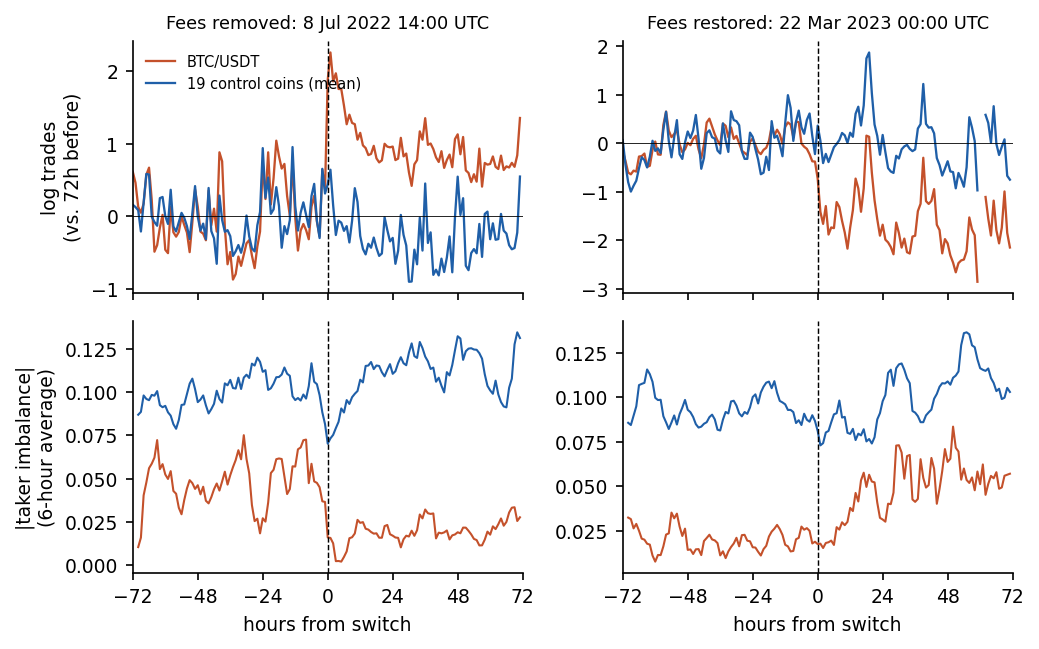
\includegraphics[width=0.95\textwidth]{fig_switch_hours.png}
\caption{Hourly trades and taker imbalance around the two fee switches. Top: log number of trades
relative to the mean over the 72 hours before the switch, for BTC/USDT and for the average of the
\feeNcontrols{} control coins. Bottom: absolute hourly taker imbalance $|2B_t-V_t|/V_t$, six-hour
moving average. The dashed lines mark the first hour without fees (left) and the first hour with
fees again (right).}
\label{fig:switch}
\end{figure}

\paragraph{Daily measures.} For each coin and day we compute, from one-minute bars, the number of
trades, the dollar volume $V$ and the average trade size; the \emph{directional volume}
$\sum_m |B_m-S_m|$ and the \emph{two-sided volume}
\begin{equation}\label{eq:twosided}
V^{\text{2s}}=\sum_m \bigl(B_m+S_m-|B_m-S_m|\bigr)=\sum_m 2\min(B_m,S_m),
\end{equation}
where $B_m$ and $S_m$ are the dollar volumes of buyer- and seller-initiated trades in minute $m$, so
that two-sided volume is the part of the day's volume that is offset by opposite aggressor flow
within the same minute; the mean absolute hourly taker imbalance; realised volatility; the Amihud
ratio from hourly bars; Kyle's lambda as the slope of one-minute returns on signed dollar flow,
with flow signed by BVC and, alternatively, observed; VPIN computed from hourly BVC-signed and from
observed signed volume; the $R^2$ of one-minute returns on observed flow; the correlation of
one-minute BVC imbalance with observed imbalance; and the first-order autocorrelation of one-minute
returns.

\paragraph{Design.} BTC/USDT is the treated unit and the \feeNcontrols{} other USDT pairs of
Section~\ref{sec:data} are the controls. For each measure let $D_d$ be the value for BTC on day $d$
minus the average over the controls (in logarithms for positive quantities), which removes
market-wide movements as day fixed effects would. The effect of a switch is the change in the mean
of $D_d$ from the 90 days before to the 90 days after it, estimated by regressing $D_d$ on an
indicator for the later window with Newey-West standard errors (30 lags); 8 July 2022, which is
split between the two regimes, is left out. With a single treated unit, conventional standard
errors can understate uncertainty \citep{conley2011}, so we add two permutation tests. In the
\emph{in-space} test each control in turn is treated as if it had been treated, with the remaining
controls as its comparison group, and the $p$-value is the rank of BTC's absolute effect among all
\panelN{} coins; the smallest attainable value is \feeMinPspace{} \citep{abadie2010}. In the
\emph{in-time} test the same statistic is computed for BTC at \feeNtime{} weekly placebo dates in
2024--2026, when no fee change affected BTC/USDT, and the $p$-value is the share of placebo effects at
least as large in absolute value. The identifying assumption is that, without the fee change, the
difference between BTC and the average control would not have shifted at the switch. The restoration
of fees provides a second, independent check: a bitcoin-specific shock that happened to coincide with
the removal of fees would have to be undone, at the same hour of the day, eight and a half months
later.

\begin{table}[t]
\centering\caption{Effects of removing and restoring fees on BTC/USDT}\label{tab:feedid}
\resizebox{\textwidth}{!}{\begin{tabular}{lrrrrrrrrr}
\toprule
 & \multicolumn{3}{c}{BTC/USDT, daily median} & \multicolumn{3}{c}{Fees removed} & \multicolumn{3}{c}{Fees restored}\\
\cmidrule(lr){2-4}\cmidrule(lr){5-7}\cmidrule(lr){8-10}Measure & Before & Zero fee & After & $\Delta$ ($t$) & $p_{\text{space}}$ & $p_{\text{time}}$ & $\Delta$ ($t$) & $p_{\text{space}}$ & $p_{\text{time}}$\\
\midrule
\multicolumn{10}{l}{\emph{Panel A. Trading activity}}\\
Trades per day (millions) & 1.12 & 5.74 & 0.82 & 1.68 (12.2) & 0.050 & 0.008 & \ensuremath{-}1.68 (\ensuremath{-}18.1) & 0.050 & 0.008\\
Dollar volume per day (\$bn) & 1.78 & 4.73 & 1.05 & 1.21 (5.9) & 0.100 & 0.008 & \ensuremath{-}1.18 (\ensuremath{-}11.2) & 0.050 & 0.008\\
Average trade size (\$) & 1,566 & 826 & 1,259 & \ensuremath{-}0.46 (\ensuremath{-}4.3) & 0.100 & 0.081 & 0.50 (7.5) & 0.050 & 0.073\\
\multicolumn{10}{l}{\emph{Panel B. Direction of the volume (one-minute taker flow)}}\\
Directional volume $\sum_m|B_m-S_m|$ (\$bn) & 0.44 & 0.55 & 0.36 & 0.43 (3.3) & 0.200 & 0.185 & \ensuremath{-}0.27 (\ensuremath{-}3.1) & 0.350 & 0.565\\
Two-sided volume (\$bn) & 1.35 & 4.20 & 0.70 & 1.43 (6.0) & 0.100 & 0.008 & \ensuremath{-}1.33 (\ensuremath{-}12.0) & 0.050 & 0.008\\
Two-sided share of volume & 0.74 & 0.88 & 0.66 & 0.16 (6.2) & 0.050 & 0.008 & \ensuremath{-}0.15 (\ensuremath{-}8.9) & 0.050 & 0.008\\
Mean $|$hourly taker imbalance$|$ & 0.065 & 0.023 & 0.086 & \ensuremath{-}1.03 (\ensuremath{-}9.3) & 0.050 & 0.008 & 1.15 (21.3) & 0.050 & 0.008\\
\multicolumn{10}{l}{\emph{Panel C. Liquidity and flow measures computed from bars}}\\
Amihud ratio, hourly bars ($|r|$ per \$bn) & 0.064 & 0.013 & 0.052 & \ensuremath{-}1.18 (\ensuremath{-}6.9) & 0.100 & 0.008 & 1.52 (21.8) & 0.050 & 0.008\\
Kyle's $\lambda$, BVC-signed flow (bps per \$M) & 3.81 & 1.53 & 3.05 & \ensuremath{-}0.39 (\ensuremath{-}3.1) & 0.150 & 0.032 & 0.97 (15.2) & 0.050 & 0.008\\
VPIN, BVC & 0.50 & 0.45 & 0.47 & \ensuremath{-}0.10 (\ensuremath{-}4.7) & 0.050 & 0.008 & 0.11 (5.1) & 0.050 & 0.008\\
\multicolumn{10}{l}{\emph{Panel D. The same quantities from observed taker flow}}\\
Kyle's $\lambda$, observed flow (bps per \$M) & 6.29 & 5.55 & 5.90 & 0.24 (1.4) & 0.400 & 0.435 & 0.30 (4.1) & 0.250 & 0.290\\
VPIN, observed flow & 0.069 & 0.023 & 0.083 & \ensuremath{-}1.08 (\ensuremath{-}8.8) & 0.050 & 0.008 & 1.11 (23.1) & 0.050 & 0.008\\
$R^2$ of 1m returns on observed flow & 0.24 & 0.41 & 0.40 & 0.13 (5.2) & 0.050 & 0.008 & \ensuremath{-}0.06 (\ensuremath{-}3.8) & 0.050 & 0.081\\
corr(BVC, observed imbalance), 1m & 0.50 & 0.59 & 0.61 & 0.05 (4.1) & 0.150 & 0.008 & \ensuremath{-}0.05 (\ensuremath{-}6.2) & 0.100 & 0.008\\
\multicolumn{10}{l}{\emph{Panel E. Prices}}\\
Realised volatility (\% per day) & 3.05 & 2.42 & 1.76 & 0.15 (1.4) & 0.900 & 0.742 & 0.48 (1.9) & 0.150 & 0.169\\
First-order autocorrelation of 1m returns & 0.012 & \ensuremath{-}0.002 & 0.016 & \ensuremath{-}0.01 (\ensuremath{-}0.5) & 0.850 & 0.677 & 0.02 (2.0) & 0.250 & 0.306\\
\bottomrule
\end{tabular}
}
\tabnote{Daily medians for BTC/USDT from 1 January to 7 July 2022 (before), 9 July 2022 to 21 March
2023 (zero fee) and 22 March to 6 September 2023 (after). $\Delta$: change in the mean of the
BTC-minus-control difference between the 90 days before and the 90 days after the switch, in log
points for the measures shown in logs (all except the two-sided share, the $R^2$, the correlation
and the autocorrelation, which are in levels), with the Newey-West $t$-statistic in parentheses.
$p_{\text{space}}$: rank of BTC's absolute effect among the \panelN{} coins when each control is
treated in turn as if it had been treated. $p_{\text{time}}$: share of \feeNtime{} placebo dates in
2024--2026 with an absolute effect at least as large.}
\end{table}

\subsection{Results}

\paragraph{Activity.} Table~\ref{tab:feedid} reports the effects. Removing fees multiplied the number
of trades on BTC/USDT by \feeOnTradesX{} and its dollar volume by \feeOnDvolX{} relative to the
controls. Both effects are larger than at any placebo date. The effect on trades is the largest among
the twenty coins; for dollar volume one control, ETC, had a larger change, as its trading surged in
July 2022 ahead of Ethereum's switch to proof of stake, which was expected to send miners to the
Ethereum Classic network. Both effects were reversed when fees returned (\feeOffTrades{} and
\feeOffDvol{} log points), and there BTC's changes are the largest of all coins. The average trade
became smaller.

\paragraph{Where the volume came from.} The new volume had little direction. Two-sided volume rose by
a factor of \feeOnTwoX{} and the two-sided share of volume by \feeOnShare. Directional volume rose by a
factor of \feeOnNetX, but this increase is not significant in either permutation test
($p_{\text{space}}=\feeOnNetPs$, $p_{\text{time}}=\feeOnNetPt$), and neither is the decline when fees
returned; some directional flow may have moved to Binance from other exchanges, whose fees did not
change. Relative to the counterfactual implied by the controls, \feeExcessTwoShare{} of the
additional dollar volume during the promotion was offset within the same minute by opposite aggressor
flow. The mean absolute hourly imbalance fell by
\feeOnImbPctA\% and recovered when fees returned. Trade-level data around the switches
(Table~\ref{tab:forensics}) show the same at a finer scale: the share of BTC/USDT volume offset by
opposite aggressor flow within the \emph{same second} was \tfBtcTwoSecA{} on the two days before the
fees were removed and \tfBtcTwoSecB{} on the two days after, and \tfBtcTwoSecC{} on the two days
before they were restored and \tfBtcTwoSecD{} after; on ETH/USDT it was between \tfEthTwoSecMin{} and
\tfEthTwoSecMax{} on all eight days. Immediate round trips of identical size, a trade followed within
one second by an opposite trade of exactly the same quantity, account for at most \tfBtcPingVolMax{}
of BTC volume on any of these days. The fee-free volume was therefore not a simple repetition of
matched orders but fast two-sided trading in varying sizes, which is what both high-frequency
liquidity provision and wash trading designed to avoid detection would produce
\citep{cong2023,aloosh2024}. Aggressor flags cannot tell the two apart.

\begin{table}[t]
\centering\caption{Trade-level composition of volume around the fee switches}\label{tab:forensics}
\resizebox{\textwidth}{!}{\begin{tabular}{llrrrrrr}
\toprule
Days & Pair & Trades (M/day) & Median trade (\$) & Round trips: trades & volume & Two-sided, 1s & Two-sided, 1m\\
\midrule
fees (before removal) & BTC/USDT & 1.17 & 250 & 1.2\% & 0.1\% & 30\% & 82\%\\
fees (before removal) & ETH/USDT & 0.63 & 470 & 0.5\% & 0.0\% & 32\% & 79\%\\
zero fees (after removal) & BTC/USDT & 3.16 & 204 & 1.4\% & 1.3\% & 59\% & 91\%\\
zero fees (after removal) & ETH/USDT & 0.46 & 285 & 3.7\% & 0.4\% & 20\% & 72\%\\
zero fees (before restoration) & BTC/USDT & 10.38 & 181 & 0.6\% & 0.1\% & 53\% & 92\%\\
zero fees (before restoration) & ETH/USDT & 0.80 & 237 & 0.2\% & 0.2\% & 25\% & 77\%\\
fees (after restoration) & BTC/USDT & 1.37 & 157 & 0.3\% & 0.1\% & 25\% & 76\%\\
fees (after restoration) & ETH/USDT & 0.68 & 343 & 0.3\% & 0.2\% & 26\% & 77\%\\
\bottomrule
\end{tabular}
}
\tabnote{Averages over two days: 6--7 July 2022 (fees), 9--10 July 2022 (zero fees), 20--21 March 2023
(zero fees) and 23--24 March 2023 (fees). Trades are Binance aggregated trades (all fills of one taker
order at one price). Round trips: share of trades, and of dollar volume, that are followed or
preceded within one second by a trade of identical quantity with the opposite aggressor side.
Two-sided: $1-\sum_s|B_s-S_s|/\sum_s(B_s+S_s)$ over seconds or minutes $s$.}
\end{table}

\paragraph{What the bars say.} Bar-based measures read the episode as a large improvement in
liquidity. The Amihud ratio fell by \feeOnAmihudPctA\% relative to the controls and Kyle's lambda
estimated from BVC-signed flow by \feeOnLamBvcPctA\%; both returned towards their earlier levels when
fees were restored. VPIN computed with BVC changed by only \feeOnVpinBvcPct\%, so a researcher using
it would conclude that the toxicity of order flow was unaffected.

\paragraph{What the observed flow says.} Observed flow tells a different story. Price impact per
dollar of observed net flow, Kyle's lambda with observed signing, changed by \feeOnLamTruePct\%
($t=\feeOnLamTrueT$, $p_{\text{space}}=\feeOnLamTruePs$, $p_{\text{time}}=\feeOnLamTruePt$) when
fees were removed and by \feeOffLamTruePct\% when they returned ($p_{\text{space}}=\feeOffLamTruePs$,
$p_{\text{time}}=\feeOffLamTruePt$), and realised volatility did not change significantly at either
switch. VPIN computed from observed flow, by contrast, fell by \feeOnVpinTruePctA\% and recovered at
the restoration: the imbalance of aggressor flow per unit of volume collapsed, because the added
volume was balanced. A dollar of net order flow moved prices at least as much as before, so liquidity
for a trader with a directional order did not improve, whatever the volume measures say; order-book
data indicate that it deteriorated, with wider spreads and less depth \citep{galati2024}. The Amihud
ratio scales price changes by gross volume and VPIN-BVC scales classified flow by gross volume;
neither can tell volume that moves prices from volume that is offset within the minute. The changes
in the Amihud ratio are roughly the sum of the changes in observed-flow lambda and in observed VPIN
(\feeOnLamTrue{} and \feeOnVpinTrue{} log points against \feeOnAmihud{} when fees were removed,
\feeOffLamTrue{} and \feeOffVpinTrue{} against \feeOffAmihud{} when they returned): most of the
movement reflects the share of net flow in volume, not the cost of price impact.

\paragraph{Calibration and information.} The episode also changes the calibration of BVC. Within the
promotion the slope of observed imbalance on hourly BVC was \BTCslopeZero, against \BTCslopeStd{}
under standard fees (Appendix Table~\ref{tab:ceiling}), so a classifier calibrated in one regime
misstates the scale of flow in the other by a factor of about four. Its correlation with observed
imbalance changed little (\feeOnCorr{} and \feeOffCorr{} at the two switches). The $R^2$ of one-minute
returns on observed flow rose by \feeOnRsq{} when fees were removed and fell by \feeOffRsqA{} when they
returned: under zero fees, net taker flow tracked contemporaneous price changes more closely, as it
would if fee-free traders, for example arbitrageurs across the thirteen bitcoin pairs, took liquidity
in the direction of price moves. For aggressor flow we therefore find no sign that zero fees made
order flow less informative about prices, the conclusion \citet{bozzetto2026} reach for order-book
imbalance; the two measures capture different flows.

\subsection{The volume follows the fee}

The strongest evidence that the two-sided volume was a response to fees, and not to anything specific
to bitcoin or to USDT, comes from the other bitcoin pairs (Figure~\ref{fig:pairs} and
Table~\ref{tab:pairs}). While all thirteen pairs were free, BTC/TUSD traded a median of
\$\pairTusdVolB{} million a day. Once it was the only free pair it traded \$\pairTusdVolC{} million,
and its mean absolute hourly imbalance fell from \pairTusdImbB{} to \pairTusdImbC, the level BTC/USDT
had shown while it was free (\pairUsdtImbB). When fees returned on BTC/TUSD in September 2023, the
volume and the same low-imbalance signature moved to BTC/FDUSD (\$\pairFdusdVolD{} million a day,
imbalance \pairFdusdImbD), while the imbalance of BTC/USDT stayed at its pre-promotion level
(\pairUsdtImbA{} before, \pairUsdtImbC{} and \pairUsdtImbD{} after). The same pattern, high volume with
almost perfectly balanced aggressor flow, appeared three times on three different pairs, each time
exactly where trading was free.

\begin{figure}[t]
\centering
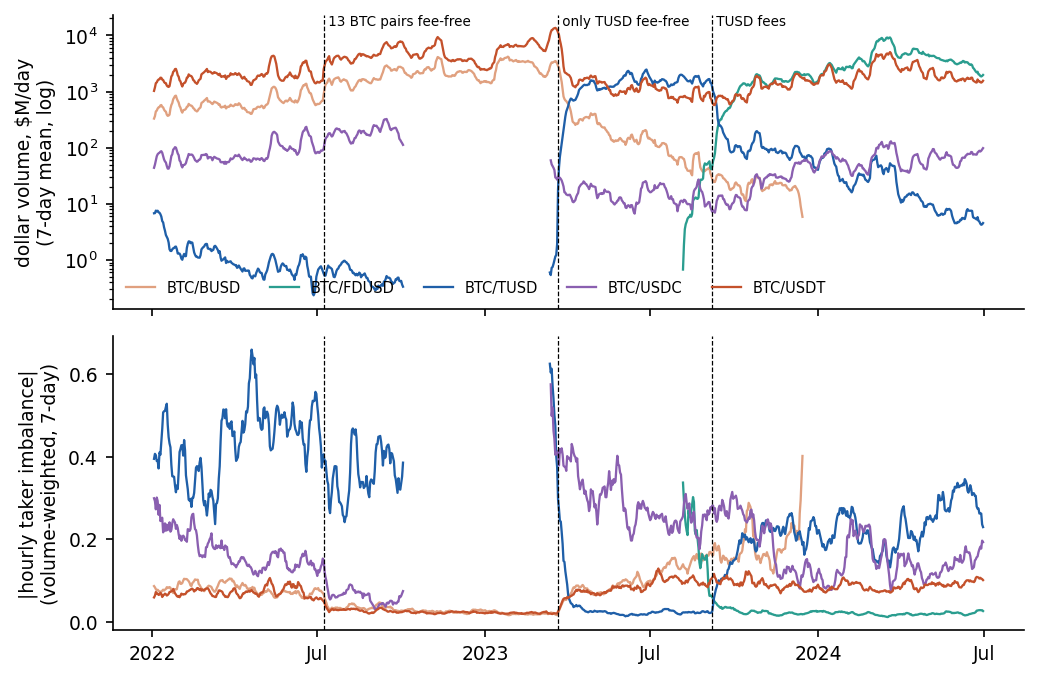
\includegraphics[width=0.95\textwidth]{fig_btc_pairs.png}
\caption{Bitcoin against five stablecoins on Binance: daily dollar volume (top, log scale) and
volume-weighted mean absolute hourly taker imbalance (bottom), seven-day moving averages. Dashed
lines: zero fees on thirteen bitcoin pairs from 8 July 2022; standard fees on all of them except
BTC/TUSD from 22 March 2023; standard fees on BTC/TUSD from 7 September 2023.}
\label{fig:pairs}
\end{figure}

\begin{table}[t]
\centering\caption{Bitcoin pairs by fee regime}\label{tab:pairs}
\resizebox{\textwidth}{!}{\begin{tabular}{lrrrrrrrr}
\toprule
 & \multicolumn{2}{c}{Jan--Jul 2022} & \multicolumn{2}{c}{Jul 2022--Mar 2023} & \multicolumn{2}{c}{Mar--Sep 2023} & \multicolumn{2}{c}{Sep--Dec 2023}\\
 & \multicolumn{2}{c}{\emph{fees on all}} & \multicolumn{2}{c}{\emph{13 pairs free}} & \multicolumn{2}{c}{\emph{only TUSD free}} & \multicolumn{2}{c}{\emph{FDUSD free}}\\
\cmidrule(lr){2-3}\cmidrule(lr){4-5}\cmidrule(lr){6-7}\cmidrule(lr){8-9}Pair & \$M/day & $|$imb.$|$ & \$M/day & $|$imb.$|$ & \$M/day & $|$imb.$|$ & \$M/day & $|$imb.$|$\\
\midrule
BTC/USDT & 1,784 & 0.072 & 4,728 & 0.024 & 1,055 & 0.086 & 1,060 & 0.091\\
BTC/BUSD & 592 & 0.080 & 2,231 & 0.027 & 132 & 0.107 & 20 & 0.196\\
BTC/TUSD & 0.9 & 0.437 & 0.5 & 0.368 & 1,419 & 0.030 & 82 & 0.196\\
BTC/FDUSD & -- & -- & -- & -- & 9.9 & 0.181 & 1,371 & 0.025\\
BTC/USDC & 71 & 0.172 & 170 & 0.101 & 13 & 0.287 & 25 & 0.195\\
\bottomrule
\end{tabular}
}
\tabnote{Median daily dollar volume (\$ million) and mean volume-weighted absolute hourly taker
imbalance of each pair, by fee regime. In the second window all five pairs were free; in the third only
BTC/TUSD was; in the fourth BTC/FDUSD was the only pair without fees. BTC/FDUSD opened in
\pairFdusdStart.}
\end{table}

\subsection{Robustness and implications}

Appendix Table~\ref{tab:feerobust} repeats the estimates with ETH/USDT as the only control, with 60-
and 180-day windows, and with a comparison of the full windows before, during and after the
promotion, with and without a linear trend in the BTC-minus-control difference. The effects on
activity, on the composition of volume and on the bar-based measures keep their sign in every
specification and are significant at the 5\% level in all but one case, the fall of BVC-based lambda
in the full-window regression with a trend. The change in observed-flow lambda, by contrast, takes
both signs across specifications. The event-study plots in Appendix Figure~\ref{fig:feeevent} show
that the effects appear and disappear at the switch dates.

Two implications follow. First, volume-based liquidity measures are not comparable across fee
regimes, exchanges or periods with different incentives to trade for its own sake. In
cryptocurrency markets, where fee promotions, volume-based fee tiers and wash trading are common
\citep{cong2023,amiram2025}, a fall in the Amihud ratio or in BVC-based lambda can mean that more
volume is being offset within the minute rather than that liquidity has improved. Second, in the
data that zero fees produce, the aggressor imbalance of a bar is diluted by two-sided trading, and
the bar's volume says little about how much of it carried direction. Exchange-reported aggressor
flow reveals the dilution; bars alone cannot.
